\begin{figure}[!t]%
    \centering
    \begin{subfigure}[t]{0.7\textwidth}
        \centering
        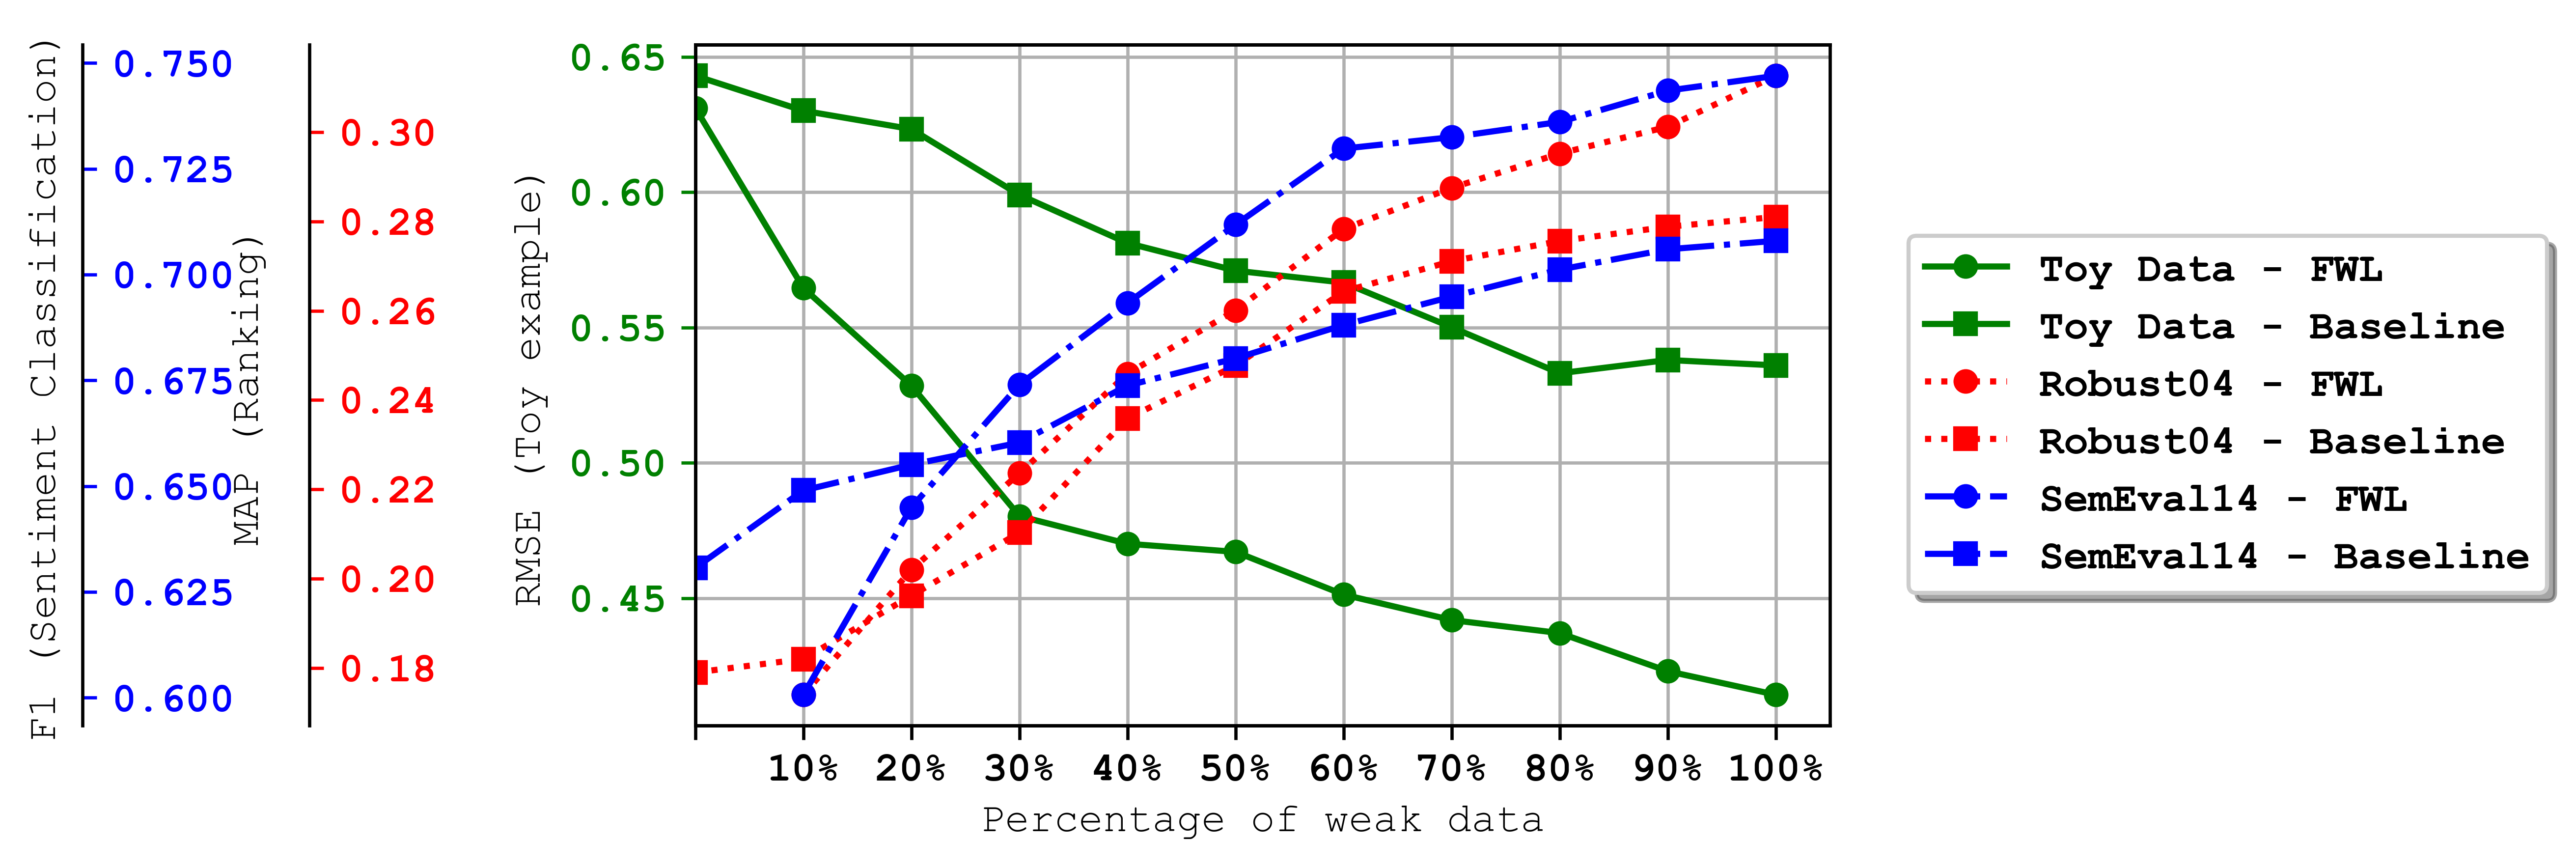
\includegraphics[width=\textwidth]{03-part-02/chapter-05/figs_and_tables/fig_data_w.png}
        \caption{\label{fig:plot_dw}\footnotesize{Models trained on different amount of weak data.}}
    \end{subfigure}%
    \hfill
    \begin{subfigure}[t]{0.7\textwidth}
        \centering
        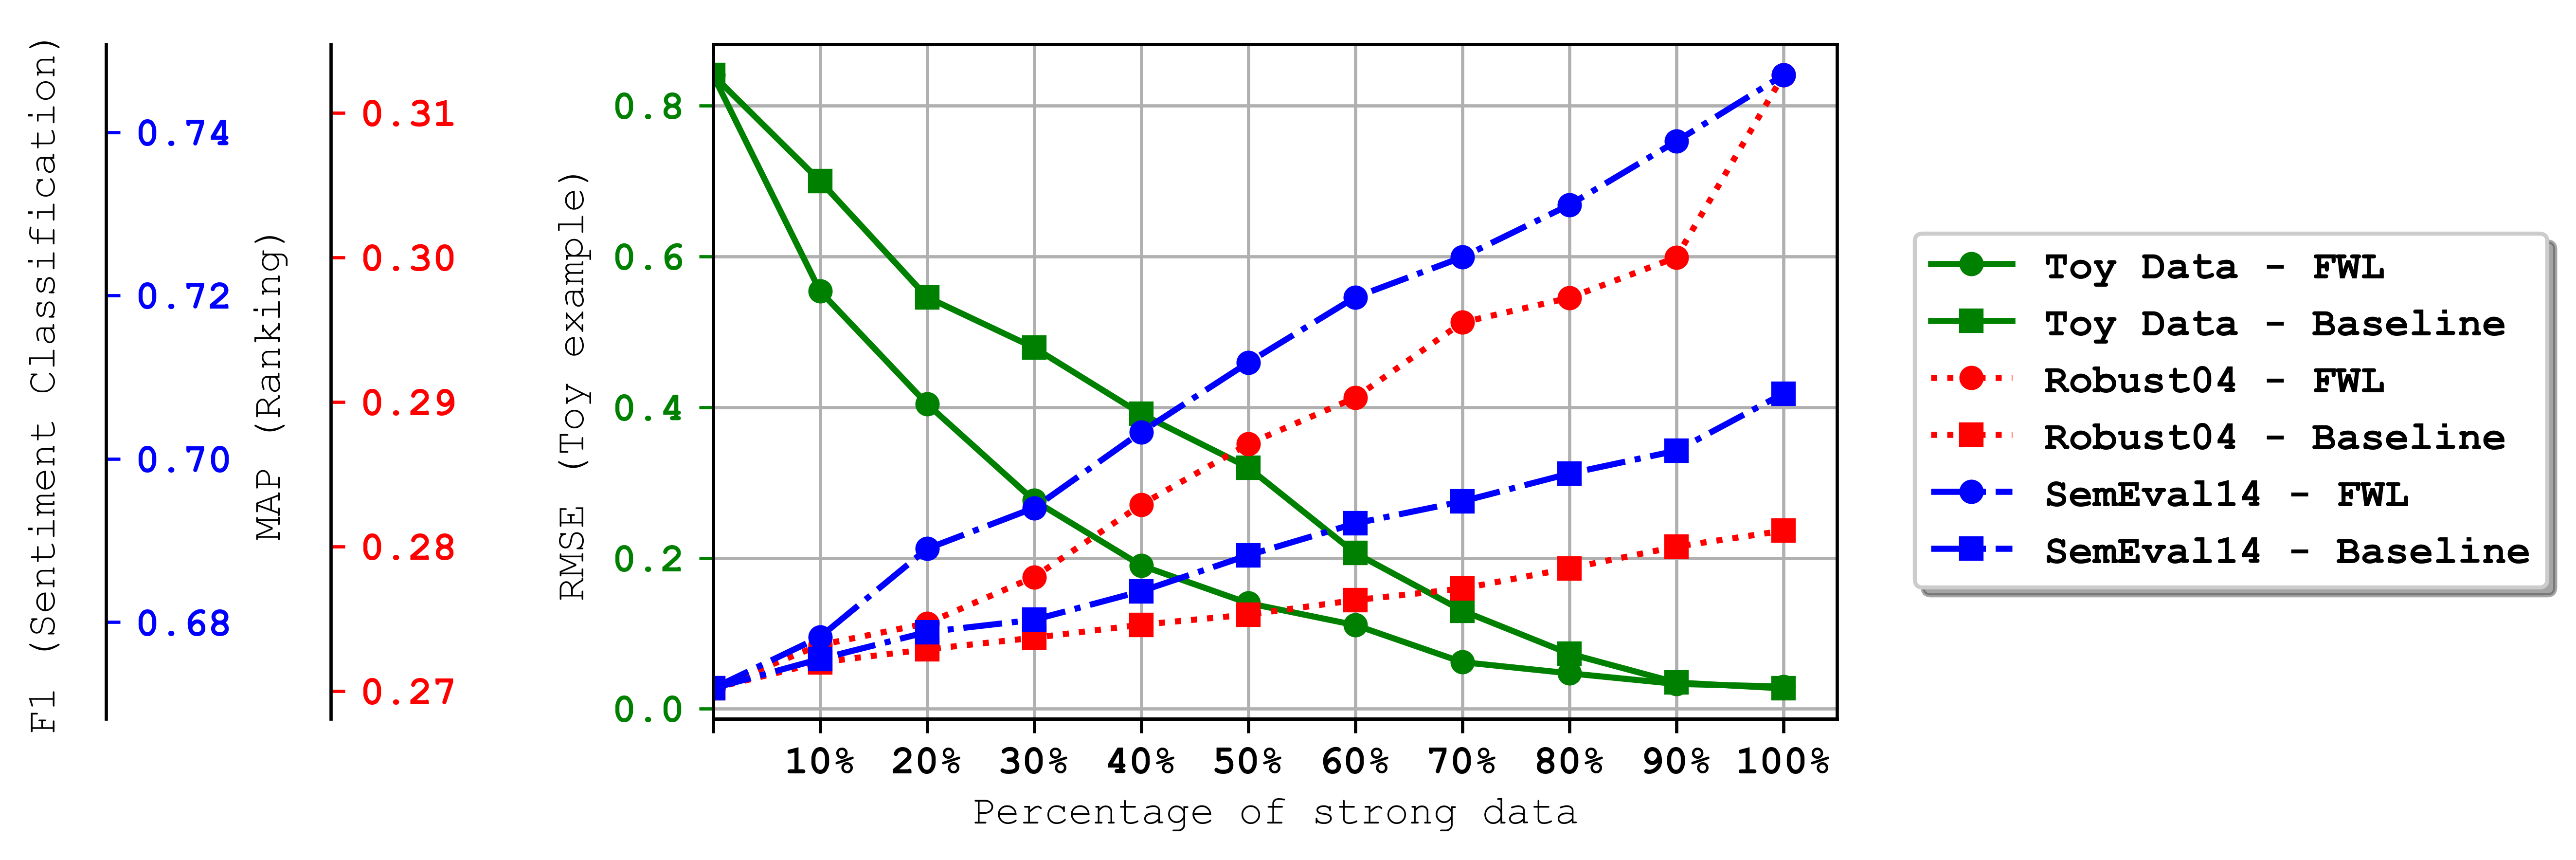
\includegraphics[width=\textwidth]{03-part-02/chapter-05/figs_and_tables/fig_data_s.png}
        \caption{\label{fig:plot_dt}\footnotesize{Models trained on different amount of strong data.}}
    \end{subfigure}%
    \caption{Performance of \fwl and the baseline model trained on different amount of data.}
    \label{fig:learning_rate}
\end{figure}